\subsubsection{ANDES}

\subsubsection{Test case: Kundur two-area system}

The Kundur two-area system is a standard benchmark network widely used for small-signal and transient stability studies.
 It was introduced in the P. Kundur power system stability literature \cite{StabilityAndControlKundur} as a compact, yet representative, test case that exposes 
 inter-area oscillatory modes and control interactions without excessive model complexity.

\begin{figure}[h!]
    \centering
    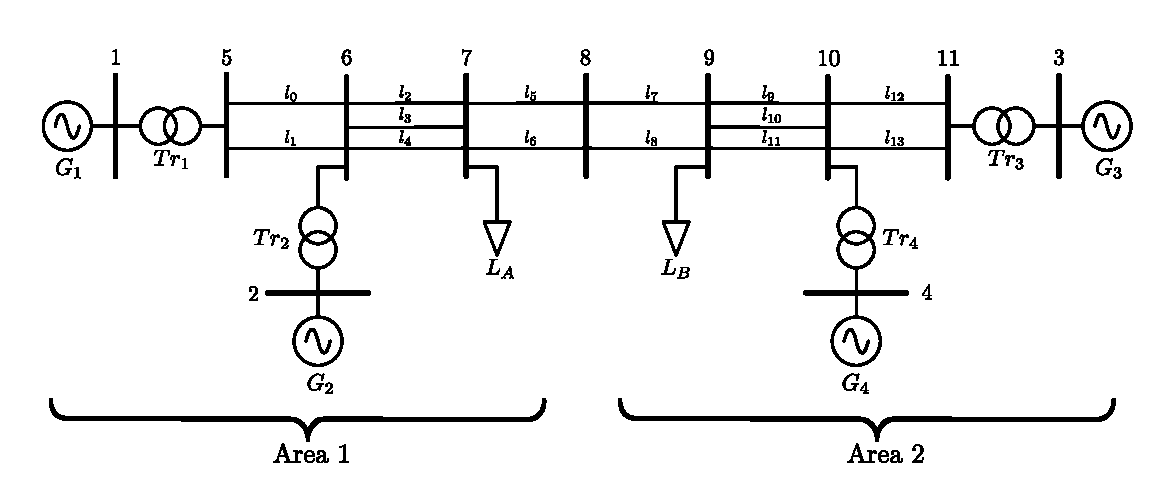
\includegraphics[width=1\linewidth]{inkscape_svg/Kundur_system_no_shunt.pdf}
    \caption{Kundur two-area system without shunt.}
    \label{fig:kundur_system}
\end{figure}

Figure \ref{fig:kundur_system} shows the one-line diagram of the Kundur two-area system without shunt. The main characteristics of the system are the following:
\begin{itemize}
    \item There are two areas connected by a pair of parallel lines. In each area, 2 synchronous generators are placed so that each area can swing against 
    each other and produce inter-area oscillations.
    \item All the synchronous generators are connected to the network through a transformer.
    \item In this version of the Kundur two-area system no shunts are connected to buses 7 and 9.
    \item While the system seems exactly symmetrical, the loads and generators are not exactly equal. This provoques the need of power exchange between areas.
\end{itemize}

Table \ref{tab:properties_kundur} summarizes the parameters of the system.

\begin{table}[H]
\centering
\caption{Main parameters of the Kundur two-area system without shunts.}
\label{tab:properties_kundur}
\renewcommand{\arraystretch}{1.2}
\small
\begin{tabular}{llcl}
\hline
\textbf{Element} & \textbf{Parameter} & \textbf{Symbol / Value} & \textbf{Units / Notes} \\ 
\hline

\multicolumn{4}{l}{\textbf{Buses}} \\ 
\hline
Bus1 to 4 & Nominal voltage & $20$ & kV \\ 
Bus5 to 11 & Nominal voltage & $230$ & kV \\ 
\hline

\multicolumn{4}{l}{\textbf{Generators}} \\ 
\hline
G1, G2 & Nominal Power & $900$ & MVA \\ 
       & Nominal voltage & $20$ & kV \\ 
       & Inertia constant & $M = 13$ & s \\ 
       & Damping coefficient & $D = 10$ & -- \\ 
       & Impedances & $r_a = 0,0$, $x_d = 0,3$ & p.u. \\ 
\hline
G3, G4 & Nominal Power & $900$ & MVA \\ 
       & Nominal voltage & $20$ & kV \\ 
       & Inertia constant & $M = 12,35$ & s \\ 
       & Damping coefficient & $D = 10$ & -- \\ 
       & Impedances & $r_a = 0,0$, $x_d = 0,3$ & p.u. \\ 
\hline

\multicolumn{4}{l}{\textbf{Transformers}} \\ 
\hline
Tr 1, 2, 3, 4 & Impedance & $R = 0,0$, $X = 0,15$, $B = 0,0$ & p.u. \\ 
               & Rate & $900$ & MVA \\ 
\hline

\multicolumn{4}{l}{\textbf{Transmission lines}} \\ 
\hline
Line 0, 1, 12, 13 & Impedance & $R = 0,005$, $X = 0,05$, $B = 0,02187$ & p.u. \\ 
                   & Rate & $750$ & MVA \\ 
\hline
Line 2, 3, 4, 9, 10, 11 & Impedance & $R = 0,003$, $X = 0,03$, $B = 0,00583$ & p.u. \\ 
                         & Rate & $700$ & MVA \\ 
\hline
Line 5, 6, 7, 8 (tie-line) & Impedance & $R = 0,011$, $X = 0,11$, $B = 0,19250$ & p.u. \\ 
                            & Rate & $400$ & MVA \\ 
\hline

\multicolumn{4}{l}{\textbf{Loads}} \\ 
\hline
Load A & Power & $P_L = 967$, $Q_L = 100$ & MW, Mvar \\ 
Load B & Power & $P_L = 1767$, $Q_L = 100$ & MW, Mvar \\ 
\hline

\end{tabular}
\end{table}

\begin{figure}[H]
  \centering
  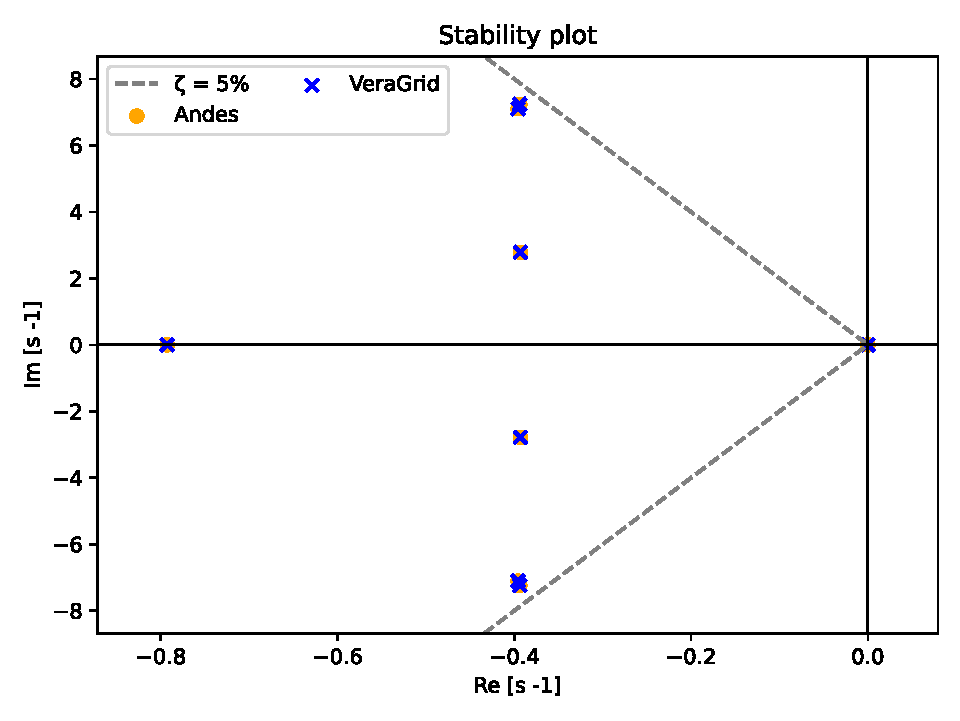
\includegraphics[width=0.8\linewidth]{inkscape_svg/andes_vs_veragrid_kundur.pdf}
  \caption{Andes vs VeraGrid complex domain plot comparison.}
  \label{fig:AndesvsVeraGrid}
\end{figure}


Figure \ref{fig:AndesvsVeraGrid} shows the comparison in the complex plane of the eigenvalues obtained
with VeraGrid and Andes for the Kundur two-area system without shunts, while Tables \ref{tab:eigenvalues_kundur} and
\ref{tab:pfacotrs_kundur} show the modes, damping ratios, oscillation frequencies and participation factors of the system.
The results between Andes and VeraGrid are practically identical, 
with less than 0,0001\% absolute error, this one due to numerical computation differences.





\begin{table}[H]
\centering
\caption{Modes, damping ratios and oscillation frequencies of the Kundur Two-Area System.}
\label{tab:eigenvalues_kundur}
\renewcommand{\arraystretch}{1.2}
\small
\begin{tabular}{lcccc}
\hline
\textbf{Mode} & \textbf{Real part} & \textbf{Imaginary part} & \textbf{Damping ratio} & \textbf{Oscillation Frequency [Hz]} \\ 
\hline
Mode 0 & -0,3938 & 7,2377 & 0,0543 & 1,1519 \\
Mode 1 & -0,3938 & -7,2377 & -- & -- \\
Mode 2 & -0,3958 & 7,1061 & 0,0556 & 1,1310 \\
Mode 3 & -0,3958 & -7,1061 & -- & -- \\
Mode 4 & -0,3931 & 2,7838 & 0,1398 & 0,4431 \\
Mode 5 & -0,3931 & -2,7838 & -- & -- \\
Mode 6 & 0,0000  & 0,0000  & -- & -- \\
Mode 7 & -0,7926 & 0,0000  & -- & -- \\
\hline
\end{tabular}
\end{table}


\begin{table}[H]
\centering
\caption{Participation factors of the Kundur Two-Area System.}
\label{tab:pfactors_kundur}
\renewcommand{\arraystretch}{1.2}
\small
\begin{tabular}{lcccccccc}
\hline
\textbf{State/Mode} & \textbf{Mode 0} & \textbf{Mode 1} & \textbf{Mode 2} & \textbf{Mode 3} & \textbf{Mode 4} & \textbf{Mode 5} & \textbf{Mode 6} & \textbf{Mode 7} \\ 
\hline
$\delta_1$ & 0,123 & 0,123 & 0,102 & 0,102 & 0,174 & 0,174 & 0,197 & 0,006 \\
$\omega_1$ & 0,123 & 0,123 & 0,102 & 0,102 & 0,174 & 0,174 & 0,000 & 0,197 \\
$\delta_2$ & 0,151 & 0,151 & 0,122 & 0,122 & 0,117 & 0,117 & 0,214 & 0,006 \\
$\omega_2$ & 0,151 & 0,151 & 0,122 & 0,122 & 0,117 & 0,117 & 0,000 & 0,214 \\
$\delta_3$ & 0,103 & 0,103 & 0,157 & 0,157 & 0,102 & 0,102 & 0,283 & 0,006 \\
$\omega_3$ & 0,103 & 0,103 & 0,156 & 0,156 & 0,102 & 0,102 & 0,000 & 0,272 \\
$\delta_4$ & 0,123 & 0,123 & 0,119 & 0,119 & 0,108 & 0,108 & 0,306 & 0,006 \\
$\omega_4$ & 0,123 & 0,123 & 0,119 & 0,119 & 0,107 & 0,107 & 0,000 & 0,293 \\
\hline
\end{tabular}
\end{table}


The eigenvalue analysis of the Kundur two-area system reveals the dynamic characteristics of the interconnected generators and 
provides insight into the nature and stability of the oscillatory modes. Each pair of complex conjugate eigenvalues corresponds to an 
electromechanical mode characterised by its frequency and damping ratio, which together define the system's response to
 small disturbances. Modes with negative real parts represent decaying oscillations, whereas a mode located at the origin 
 corresponds to the uniform rotation of all machines, a neutral condition that does not compromise stability. 
 The participation factors, which quantify the contribution of each state variable to every mode, enable the identification of the 
 physical components responsible for each dynamic behaviour.

The local modes are associated with oscillations of generators within the same area against one another. 
In this case, two pairs of complex conjugate eigenvalues located at $-0,3938 \pm j7,2377$ and $-0,3958 \pm j7,1061$ correspond to frequencies
 of $1,1519$ and $1,1310$~Hz with damping ratios near $5,5\%$. These modes involve mainly the rotor angles and 
 speeds of generators within each area, indicating local electromechanical interactions between closely coupled machines. 
 The relatively low damping (just above the threshold 5\%) means that oscillations at these frequencies would decay slowly after a 
 disturbance, and therefore these modes are usually targeted for improvement through power system stabilisers designed to increase 
 the effective damping while maintaining the natural frequency range around one hertz.

The inter-area mode, represented by the eigenvalue pair $-0,3931 \pm j2,7838$, exhibits a frequency of  $0,4431$~Hz and a damping 
ratio of $13,98\%$. The participation factors show that the mode involves the collective motion of generators in one area oscillating 
against those in the other, with all machines in each group moving coherently. This behaviour reflects the exchange of power 
through the tie-line connecting the two subsystems, which gives rise to slow, large-scale oscillations of the inter-area type. 
The relatively higher damping compared with the local modes suggests that the tie-line and the automatic voltage regulators 
contribute sufficient stabilising torque under the present operating point. Nevertheless, variations in power transfer or network 
strength could reduce this damping and make the inter-area oscillation more critical, as observed in many large interconnected grids.

Among the real modes, one negative value mode at approximately $-0,7926$ represents a non-oscillatory but fast-decaying mode, 
mainly related to the mechanical dynamics of the generating units. Its time constant ($\tau = 1/Re(\lambda)$), around $1,26$~s, indicates a rapid stabilising
effect that brings the system back to equilibrium after active-power mismatches or primary control actions. This mode is considered 
dominant in the sense that it governs the short-term return to balance but does not limit the overall stability margins of the system.

Finally, the eigenvalue located at the origin, $\lambda = 0$, corresponds to the uniform or rigid-body mode. 
Mathematically, it indicates marginal stability, as perturbations projected onto this mode neither grow nor decay.
Physically, however, it simply reflects the absence of an absolute angular reference: if all generator rotor angles are shifted by the same constant, 
the electrical state of the system remains unchanged. Only differences in rotor angles carry physical meaning, so this mode has no effect on the stability 
of the relative motion among machines. In practical studies, this degree of freedom is removed by selecting a reference machine or imposing a condition on 
the sum of the rotor angles, which eliminates the zero eigenvalue from the dynamic model. Consequently, although the rigid-body mode is formally marginally 
stable, it is not regarded as a sign of instability in the power system.

Overall, the eigenvalue spectrum indicates that the Kundur two-area system is dynamically stable under the studied conditions. 
The local modes show limited damping and would benefit from supplementary control, while the inter-area mode remains acceptably damped. 
The rigid-body mode is a physical artefact of the reference frame and not a true stability concern. These results are consistent with the 
classical interpretation of the two-area system and confirm its suitability as a benchmark for electromechanical oscillation studies.



